\documentclass{beamer}
\usepackage[utf8]{inputenc}

%\usetheme{Madrid}
\setbeameroption{show notes}
\beamertemplatenavigationsymbolsempty
\hypersetup{hidelinks}

\usepackage{listings}
\lstset{language=[ISO]C++,
        basicstyle=\ttfamily\scriptsize,
        keywordstyle=\color{blue},
        stringstyle=\color{red},
        commentstyle=\color{green},
        frame=single,
        showspaces=false,
        showstringspaces=false,
        morekeywords={noexcept},
        }

\lstdefinelanguage{cmake}
{
  morekeywords=
  {
    add_executable, target_link_libraries, add_test,
  },
}

\usepackage{lmodern}
\usepackage{color}
\usepackage[backend=biber]{biblatex}
\bibliography{script}

\title{Advanced programming}
\author{David Schneider}
\date{2017}

\AtBeginPart{\frame{\partpage}\frame{\frametitle{Content Part
\insertpart}\tableofcontents}}

\begin{document}

\frame{\titlepage}

\part{Overview}

\section{Über mich}

\begin{frame}{Über mich}
\begin{block}{Name}
David Schneider
\end{block}

\begin{block}{Kontakt}
E-Mail: \url{david.schneider@fhwn.ac.at}
\end{block}

\end{frame}

\begin{frame}{Erfahrungen}

\begin{block}{Ausbildung}
\begin{itemize}
  \item Elektroniker Lehre mit Berufsmatura
  \item Zürcher Fachhochschule, Elektrotechnik, Vertiefung Regelungstechnik und
Computertechnik
\end{itemize}
\end{block}

\begin{block}{Berufserfahrung}
\begin{itemize}
  \item Messsystem für hochprezise Temperaturmessung, IST AG
  \item Message Gateway für SMS, Dimoco
  \item Automotiv Steuergeräte für Scheinwerfer, ZKW
\end{itemize}
\end{block}

\end{frame}

\section{Overview}

%%%%%%%%%%%%%%%%%%%%%%%%%%%%%%%%%%%%%%%%%%%%%%%%%%%%%%%%%%%%%%%%%%%%%
\begin{frame}{Modalitäten}
\begin{description}
\item[Umfang] 5 ECTS (45 Lektionen = 34h, Total 125h)
\item[Lehr- und Lernformen]: Vorlesung mit integrierter Übung
\item[Prüfungsmodalitäten]: LV-abschließende Prüfung; Übung, Arbeit
\end{description}
\end{frame}

%%%%%%%%%%%%%%%%%%%%%%%%%%%%%%%%%%%%%%%%%%%%%%%%%%%%%%%%%%%%%%%%%%%%%
\begin{frame}{Lehrinhalte}
Erlernen von Konzepten der objektorientierten Programmierung anhand der
Programmiersprache C++ (Klassen und Objekte, Kapselung, Vererbung und
Polymorphismus), Fehler- und Ausnahmebehandlung, Coding Guidelines, Design
Patterns, Design for Testability. Bildung von Modellen, Abstraktion,
Lösungsfindung und Evaluation in der  objektorientierten Programmierung.
Einbindung vorhandener Lösungskonzepte und systematische Herangehensweise an
konkreten Problemstellungen.
\end{frame}

%%%%%%%%%%%%%%%%%%%%%%%%%%%%%%%%%%%%%%%%%%%%%%%%%%%%%%%%%%%%%%%%%%%%%
\begin{frame}{Literaturempfehlungen}
\begin{itemize}
\item E. Gamma et al., Design Patterns, Addison-Wesley (1995)
\item R. Martin, Clean Code, Prentice Hall Pearson Education (2009)
\item B. Stroustrup: The C++ Programming Language, 4th edition, Addison Wesley
(2013)
\item A. Alexandrescu: Modern C++ Design, Addison Wesley (2001)
\item H. Sutter: C++ Coding Standards, Addison Wesley (2004)
\end{itemize}
\end{frame}

\begin{frame}{Themen}
\begin{itemize}
  \item Objekt-Orientieres Design
  \item Einführung in C++
  \item Clean Code
  \item Unit Testing
  \item Software Development Methodology
  \item Coding Standards
\end{itemize}
\end{frame}

\begin{frame}{Benotung}
\begin{itemize}
  \item Schriftliche Prüfung (60 Punkte)
  \item Übung: Programming Idiom (30 Punkte)
  \item Projektarbeit (60 Punkte)
\end{itemize}
Für eine positive Beurteilung sind insgesamt 80 Punkte erforderlich.
\end{frame}

\begin{frame}{Termine 2017}
\begin{table}
\begin{tabular}{l | l | l }
Datum & Raum \\
\hline
22. September 2017 & EDV9 \\
29. September 2017 & EDV6 \\
06. Oktober 2017 & EDV6 \\
20. Oktober 2017 & EDV6 \\
03. November 2017 & EDV6 & Abgabe Übung\\
10. November 2017 & EDV6 \\
17. November 2017 & EDV6 \\
24. November 2017 & EDV6 \\
01. Dezember 2017 & EDV8 & Fertigstellen und Abgabe Arbeit\\
15. Dezember 2017 & EDV6 & Schriftliche Prüfung
\end{tabular}
\end{table}
\end{frame}

%\begin{frame}{Gegrüfte Themen}
%\begin{itemize}
%  \item C++ Tutorial
%  \item Pattern (Factory Method, Builder, Singleton, Command, Observer,
%  Visitor)
%  \item SOLID
%  \item Testing
%  \item Code Smells
%  \item Coding Standards
%\end{itemize}
%\end{frame}

\begin{frame}
Wer verfügt über grundlegende Programmierkentnisse?
\end{frame}

\begin{frame}
Welche Programmiersprachen kennen/beherschen Sie?
\end{frame}

\begin{frame}{Levels der Software Entwicklung}
\textbf{LEVEL1:} Das Programm funktioniert \\
\textbf{LEVEL2:} Das Programm ist veränderbar/erweiterbar \\
\textbf{LEVEL3:} Teile der Software sind wiederverwendbar
\end{frame}

\section{Einstufung}
\begin{frame}[fragile]{Frage 1}
Was ist die Ausgabe von folgendem Code:
\begin{lstlisting}
for (int i = 0; i < 5; ++i)
{
  std::cout << i << std::endl;
}
\end{lstlisting}
\end{frame}

\begin{frame}[fragile]{Frage 2}
Was ist der Typ und der Wert des folgenden Ausdrucks?
\begin{lstlisting}
int x = 12;
int y = 7;

(x != 4) || (y == 2)
\end{lstlisting}
\end{frame}

\begin{frame}[fragile]{Frage 3}
Was ist der Inhalt der Variablen str und p?
\begin{lstlisting}
char str[10] = "Hello";
char *const p = &str[1];
*p = 'a';
\end{lstlisting}
\end{frame}

\begin{frame}[fragile]{Frage 4}
Was ist der Unterschied zwischen Step-Over und Step-Into (im Debugger)?
\end{frame}

\section{Lösungen}
\begin{frame}[fragile]{Frage 1}
Was ist die Ausgabe von folgendem Code:
\begin{lstlisting}
for (int i = 0; i < 5; ++i)
{
  std::cout << i << std::endl;
}
\end{lstlisting}

\begin{lstlisting}
0
1
2
3
4
\end{lstlisting}
\end{frame}

\begin{frame}[fragile]{Frage 2}
Was ist der Typ und der Wert des folgenden Ausdrucks?
\begin{lstlisting}
int x = 12;
int y = 7;

(x != 4) || (y == 2)
\end{lstlisting}
Typ: boolean

Wert: true
\end{frame}

\begin{frame}[fragile]{Frage 3}
Was ist der Inhalt der Variablen str und p?
\begin{lstlisting}
char str[10] = "Hello";
char *const p = &str[1];
*p = 'a';
\end{lstlisting}

str:
\textquotedblleft{}Hallo\textbackslash0\textbackslash0\textbackslash0
                      \textbackslash0\textbackslash0\textquotedblright

p: Adresse des zweiten Zeichens in str
\end{frame}

\begin{frame}[fragile]{Frage 4}
Was ist der Unterschied zwischen Step-Over und Step-Into (im Debugger)?

Step-Over: Führt den gesamten anstehenden Befehl (Ausdruck) aus. Der Programm
Zähler steht auf dem nächsten Befehl.

Step-Into: Ist der anstehende Befehl ein Funktionsaufruf, wird das Programm 
bis zum ersten Befehl in der Funktion ausgeführt.
\end{frame}


\part{Introduction}

\section{Introduction}

\subsection{C++}
\begin{frame}{C++ - Overview}
\begin{itemize}
  \item compiled language
  \item general-purpose programming language
  \item Multi-pradigma
  \begin{itemize}
    \item procedural
    \item functional
    \item object-oriented
    \item generic
  \end{itemize}
  \item statically typed
  \item allows low-level memory manipulation
  \item designed for large, resource constrained systems 
\end{itemize}
\end{frame}


\begin{frame}{C++ - Standardization}
\itemize{}
\item[1979] C with Classes first implemented 
\item[1998] C++98 (ISO/IEC 14882:1998)
\item[2003] C++03 (ISO/IEC 14882:2003)
\item[2011] C++11 (ISO/IEC 14882:2011)
\item[2014] C++14 (ISO/IEC 14882:2014)
\item[2017] C++17 (also called C++1z)
\end{frame}

\begin{frame}{The Boost Library}
\begin{itemize}
  \item Started arround 1999
  \item several Boost libraries have been accepted for incorporation into the
  C++11 standard.
\end{itemize}
\end{frame}

\begin{frame}{Emedded Systems}
\begin{itemize}
  \item Embedded C++ (still in use?)
  \item Adaptive AUTOSAR
\end{itemize}
\end{frame}


\subsection{Object-oriented programming}

\begin{frame}{Pradigma}
OOP is a programming paradigm
\begin{block}{Objects contain}
\begin{itemize}
\item data (ak. attribute)
\item code (ak. methods)
\end{itemize}
\end{block}
\end{frame}

\begin{frame}{OOP vs. Procedural}

\begin{block}{Procedural}
data tends to be highly decoupled from the functions that operate on it
\end{block}

\begin{block}{Object-oriented}
data tends to carry with it a collection of functions
\end{block}

\end{frame}

\subsection{Object-oriented concepts}

\begin{frame}{Classes and objects}

\begin{block}{Class}
The blueprint for an object. Defines how a object should be created.
\end{block}

\begin{block}{Object}
An instance of a class. Gets created during runtime.
\end{block}

\end{frame}

\begin{frame}{Information hidding}
Encapsulate data and hide the internal structure from caller. This allows
changing the internal details without affecting.
\end{frame}

\begin{frame}{Inheritance}
Inheritance is when a class is based on another class, using the same
implementation to maintain the same behavior.
Such an inherited class is called a subclass of its parent class or super class.
It is a mechanism for code reuse and to allow independent extensions of the
original software via public classes and interfaces.
 Often called a `Is-A-Relation`.
\end{frame}

\begin{frame}{Interface}
Define a method without implementing it as an interface to be used by other
classes. \\
A interface is often called `an abstract base class`.
\end{frame}

\begin{frame}{Polymorphism}
\framesubtitle{aka Subtyping}
Polymorphism is the provision of a single interface to entities of different
types.

Define a implementation for a specialized type. Or change the behavior of a
class by subtyping it and overwrite a method.
\end{frame}

\part{C++ Tutorial}{cpp-tutorial}

\begin{frame}{Source}
C++ Language Tutorial
Source: \url{http://www.cplusplus.com/doc/tutorial/}
\begin{block}

reference on cplusplus.com contains some errors,
\url{http://stackoverflow.com/questions/6520052/whats-wrong-with-cplusplus-com}
\end{block}
\end{frame}

\section{Basics}

%%%%%%%%%%%%%%%%%%%%%%%%%%%%%%%%%%%%%%%%%%%%%%%%%%%%%%%%%%%%%%%%%%%%%
\begin{frame}[fragile]{Identifiers}
\begin{itemize}
  \item case-sensitive
  \item sequence of one or more letters, digits, or underscore
  \item always begin with a letter
  \item begin with underscore allowd, but used for special cases
  \item many reserved keywords, which can't be used as identifiers 
\end{itemize}
\begin{lstlisting}[caption=Identifiers Examples]
aNumber
my1st_variable
SomeMoreIdentifier
\end{lstlisting}
\end{frame}

%%%%%%%%%%%%%%%%%%%%%%%%%%%%%%%%%%%%%%%%%%%%%%%%%%%%%%%%%%%%%%%%%%%%%
\begin{frame}{Fundamental data types}
\begin{itemize}
  \item Character types
  \item Numerical integer types
  \item Floating-point types
  \item Boolean type
\end{itemize}
\end{frame}

%%%%%%%%%%%%%%%%%%%%%%%%%%%%%%%%%%%%%%%%%%%%%%%%%%%%%%%%%%%%%%%%%%%%%
\begin{frame}{Fundamental data types}
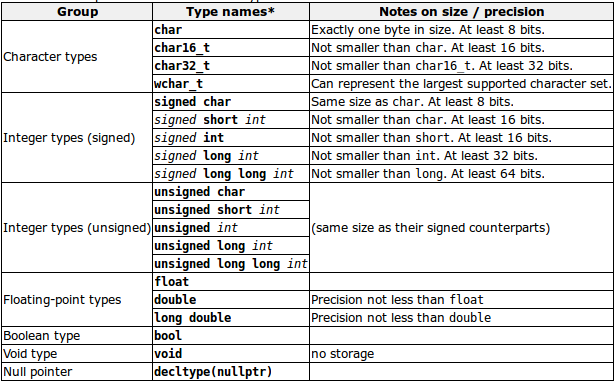
\includegraphics[scale=0.48]{img/FundamentalTypes.png}
\end{frame}

%%%%%%%%%%%%%%%%%%%%%%%%%%%%%%%%%%%%%%%%%%%%%%%%%%%%%%%%%%%%%%%%%%%%%
\begin{frame}[fragile]{Declaration of variables}
\begin{itemize}
  \item Strongly typed
  \item Every variable to be declared before first use
\end{itemize}
\begin{lstlisting}[caption=Variable declaration]
int aNumber;
float aFloatingPointerNumber;
\end{lstlisting}
\end{frame}

%%%%%%%%%%%%%%%%%%%%%%%%%%%%%%%%%%%%%%%%%%%%%%%%%%%%%%%%%%%%%%%%%%%%%
\begin{frame}[fragile]{Initialization of variables}
\begin{definition}{Initialization}
   Set the value of variable during declaration. 
\end{definition}
\begin{lstlisting}[caption=Variable initialization]
int aNumber = 5;
float aFloatingPointerNumber(6);
\end{lstlisting}
\end{frame}

%%%%%%%%%%%%%%%%%%%%%%%%%%%%%%%%%%%%%%%%%%%%%%%%%%%%%%%%%%%%%%%%%%%%%
\begin{frame}[fragile]{Type deduction: auto and decltype}
Automatic type determination with keyword `auto`.

Usefull for cases where the explicitly type is not so importent or the type is
so complex (ex. with templates) that it's hard the define the type correct.

\lstinputlisting[caption=Auto Type]{lst/AutoType.cpp}

\end{frame}

%%%%%%%%%%%%%%%%%%%%%%%%%%%%%%%%%%%%%%%%%%%%%%%%%%%%%%%%%%%%%%%%%%%%%
\begin{frame}{Introduction to strings}
Example for compound types: std::string

\lstinputlisting[caption=String Example]{lst/SimpleString.cpp}

\end{frame}


\subsection{Constants}

%%%%%%%%%%%%%%%%%%%%%%%%%%%%%%%%%%%%%%%%%%%%%%%%%%%%%%%%%%%%%%%%%%%%%
\begin{frame}[fragile]{Literals}

\begin{lstlisting}[caption=Integer Numerals]
75         // decimal
0113       // octal
0x4b       // hexadecimal
\end{lstlisting}

\end{frame}

%%%%%%%%%%%%%%%%%%%%%%%%%%%%%%%%%%%%%%%%%%%%%%%%%%%%%%%%%%%%%%%%%%%%%
\begin{frame}[fragile]{Literals}

\begin{lstlisting}[caption=Floating Point Numerals]
3.14159    // 3.14159
6.02e23    // 6.02 x 10^23
1.6e-19    // 1.6 x 10^-19
3.0        // 3.0
\end{lstlisting}

\end{frame}

%%%%%%%%%%%%%%%%%%%%%%%%%%%%%%%%%%%%%%%%%%%%%%%%%%%%%%%%%%%%%%%%%%%%%
\begin{frame}{Literals}
\begin{table}
\begin{tabular}{l | c}
Suffix & Type modifier \\
\hline
u or U & unsigned \\
l or L & long \\
ll or LL & long long \\
f or F & float \\
l or L & long double
\end{tabular}
\caption{Type modifier}
\end{table}

\end{frame}

%%%%%%%%%%%%%%%%%%%%%%%%%%%%%%%%%%%%%%%%%%%%%%%%%%%%%%%%%%%%%%%%%%%%%
\begin{frame}[fragile]{Character and string literals}
\begin{description}
\item[Character] A singel character, between single quotes
\item[String] Null-terminated string, between double quotes 
\end{description}
\begin{lstlisting}[caption=Character and string literals]
'z'
'p'
"Hello world"
"How do you do?"
\end{lstlisting}

\end{frame}

%%%%%%%%%%%%%%%%%%%%%%%%%%%%%%%%%%%%%%%%%%%%%%%%%%%%%%%%%%%%%%%%%%%%%
\begin{frame}[fragile]{Other literals}
\begin{description}
\item[Boolean] true and false
\item[Null-Pointer] reserved value to indicated, that a pointer doesn't refer to
a valid object
\end{description}
\begin{lstlisting}[caption=Other literals]
bool foo = true;
bool bar = false;
int* p = nullptr;
\end{lstlisting}
\end{frame}

%%%%%%%%%%%%%%%%%%%%%%%%%%%%%%%%%%%%%%%%%%%%%%%%%%%%%%%%%%%%%%%%%%%%%
\begin{frame}[fragile]{Typed constant expressions}
\begin{lstlisting}[caption=Typed constant expressions]
const double pi = 3.1415926;
const char tab = '\t';
\end{lstlisting}
\end{frame}

%%%%%%%%%%%%%%%%%%%%%%%%%%%%%%%%%%%%%%%%%%%%%%%%%%%%%%%%%%%%%%%%%%%%%
\begin{frame}[fragile]{Preprocessor definitions}
\begin{lstlisting}[caption=Preprocessor definitions]
#define PI 3.14159
#define NEWLINE '\n'
\end{lstlisting}
\end{frame}


\subsection{Operators}

\begin{frame}[fragile]{Assignment operator}
\begin{definition}
The assignment operator assigns a value to a variable.
\end{definition}

\begin{lstlisting}[caption=Assignment operator]
a = 5;
\end{lstlisting}

\end{frame}

%%%%%%%%%%%%%%%%%%%%%%%%%%%%%%%%%%%%%%%%%%%%%%%%%%%%%%%%%%%%%%%%%%%%%
\begin{frame}[fragile]{Arithmetic operators}
\begin{table}
\begin{tabular}{l | l}
operator & description \\
\hline
+ & addition \\
- & subtraction \\
* & multiplication \\
/ & division \\
\% & modulo
\end{tabular}
\caption{Arithmetic operators}
\end{table}
\begin{lstlisting}[caption=Modulo operator]
a = 11 % 3;
\end{lstlisting}
\end{frame}

%%%%%%%%%%%%%%%%%%%%%%%%%%%%%%%%%%%%%%%%%%%%%%%%%%%%%%%%%%%%%%%%%%%%%
\begin{frame}[fragile]{Compound assignment}
\begin{table}
\begin{tabular}{l | l}
expression & equivalent to... \\
\hline
y += x; & y = y + x; \\
x -= 5; & x = x - 5; \\
x /= y; & x = x / y; \\
price *= units + 1; & price = price * (units+1);
\end{tabular}
\caption{Compound assignment}
\end{table}
\begin{lstlisting}[caption=Modulo operator]
a += 2;   // equivalent to a=a+2
\end{lstlisting}
\end{frame}

%%%%%%%%%%%%%%%%%%%%%%%%%%%%%%%%%%%%%%%%%%%%%%%%%%%%%%%%%%%%%%%%%%%%%
\begin{frame}{Increment and decrement}
\begin{table}
\begin{tabular}{l | l}
operator & description \\
\hline
++ & increase operator \\
-- & decrease operator
\end{tabular}
\end{table}

%%%%%%%%%%%%%%%%%%%%%%%%%%%%%%%%%%%%%%%%%%%%%%%%%%%%%%%%%%%%%%%%%%%%%
\begin{table}
\begin{tabular}{l | l}
prefix & modifies the variable after evaluating \\
postfix & modifies the variable before evaluating
\end{tabular}
\end{table}
\end{frame}

%%%%%%%%%%%%%%%%%%%%%%%%%%%%%%%%%%%%%%%%%%%%%%%%%%%%%%%%%%%%%%%%%%%%%
\begin{frame}{Relational and comparison operators}
\begin{table}
\begin{tabular}{l | l}
operator & description \\
\hline
== & Equal to \\
!= & Not equal to \\
\textless & Less than \\
\textgreater & Greater than \\
\leq & Less than or equal to \\
\geq & Greater than or equal to
\end{tabular}
\caption{Relational and comparison operators}
\end{table}
\end{frame}

%%%%%%%%%%%%%%%%%%%%%%%%%%%%%%%%%%%%%%%%%%%%%%%%%%%%%%%%%%%%%%%%%%%%%
\begin{frame}{Logical operators}
\begin{table}
\begin{tabular}{l | l}
operator & description \\
\hline
\&\& & logical-and \\
\textbar\textbar & logical-or \\
! & logical-not
\end{tabular}
\caption{Logical operators}
\end{table}
\end{frame}

%%%%%%%%%%%%%%%%%%%%%%%%%%%%%%%%%%%%%%%%%%%%%%%%%%%%%%%%%%%%%%%%%%%%%
\begin{frame}{Bitwise operators}
\begin{table}
\begin{tabular}{l | l}
operator & description \\
\hline
\& & Bitwise AND \\
\textbar & Bitwise inclusive OR \\
\textasciitilde & Unary complement (bit inversion) \\
\textless\textless & Shift bits left \\
\textgreater\textgreater & Shift bits right
\end{tabular}
\caption{Bitwise operators}
\end{table}
\end{frame}

%%%%%%%%%%%%%%%%%%%%%%%%%%%%%%%%%%%%%%%%%%%%%%%%%%%%%%%%%%%%%%%%%%%%%
\begin{frame}[fragile]{Explicit type casting operator}
\begin{lstlisting}[caption=Type cast]
uint16_t a;
uint16_t b;

uint32_t sum = (uint32_t)a + b;
\end{lstlisting}
\end{frame}

%%%%%%%%%%%%%%%%%%%%%%%%%%%%%%%%%%%%%%%%%%%%%%%%%%%%%%%%%%%%%%%%%%%%%
\begin{frame}{Precedence of operators}
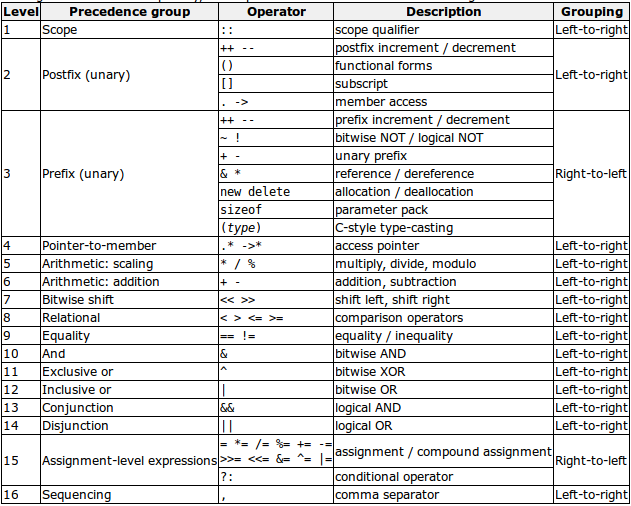
\includegraphics[scale=0.48]{img/OperatorPrecedence.png}
\end{frame}


\subsection{Basic Input/Output}

%%%%%%%%%%%%%%%%%%%%%%%%%%%%%%%%%%%%%%%%%%%%%%%%%%%%%%%%%%%%%%%%%%%%%
\begin{frame}{Streams}
\begin{itemize}
\item Abstraction `Streams` for input and output operations
\item Media independed (examples: file, consol, socket)
\item streams are a source/destination of characters
\item characters are provided/accepted sequentially
\end{itemize}
\end{frame}

%%%%%%%%%%%%%%%%%%%%%%%%%%%%%%%%%%%%%%%%%%%%%%%%%%%%%%%%%%%%%%%%%%%%%
\begin{frame}{Standard libray streams}
\begin{table}
\begin{tabular}{l | l}
stream & description \\
\hline
cin & standard input stream \\
cout & standard output stream \\
cerr & standard error (output) stream \\
clog & standard logging (output) stream \\
\end{tabular}
\caption{Bitwise operators}
\end{table}
\end{frame}

%%%%%%%%%%%%%%%%%%%%%%%%%%%%%%%%%%%%%%%%%%%%%%%%%%%%%%%%%%%%%%%%%%%%%
\begin{frame}[fragile]{Standard output (cout)}
\begin{lstlisting}[caption=Standard output]
// prints Output sentence on screen
std::cout << "Output sentence" 

// prints number 120 on screen
std::cout << 120;

// prints the value of x on screen
std::cout << x;
\end{lstlisting}
\end{frame}

%%%%%%%%%%%%%%%%%%%%%%%%%%%%%%%%%%%%%%%%%%%%%%%%%%%%%%%%%%%%%%%%%%%%%
\begin{frame}[fragile]{New line}
\begin{lstlisting}[caption=Use ASCII newline character]
std::cout << "First sentence.\n";
std::cout << "Second sentence.\nThird sentence.";
\end{lstlisting}

\begin{lstlisting}[caption=Use portable endl]
std::cout << "First sentence." << std::endl;
std::cout << "Second sentence." << std::endl
          << "Third sentence.";
\end{lstlisting}
\end{frame}

%%%%%%%%%%%%%%%%%%%%%%%%%%%%%%%%%%%%%%%%%%%%%%%%%%%%%%%%%%%%%%%%%%%%%
\begin{frame}[fragile]{Standard input (cin)}
\begin{itemize}
\item Input is only processed after `ENTER` key pressed
\item If conversion fails, not value is assigned
\item Spaces are always consideres as value terminator, which makes it difficult
to read a whole sentense into a string
\end{itemize}

\begin{lstlisting}[caption=Standard input]
int i;
std::cout << "Please enter an integer value: ";
std::cin >> i;
std::cout << "The value you entered is " << i;
std::cout << " and its double is " << i*2 << "." 
          << std::endl;
\end{lstlisting}
\end{frame}


\section{Program structure}

%%%%%%%%%%%%%%%%%%%%%%%%%%%%%%%%%%%%%%%%%%%%%%%%%%%%%%%%%%%%%%%%%%%%%
\begin{frame}[fragile]{Single statment vs. compound statement}
Where ever a single statement can be used, also a compound statement (block) can
be inserted.  compound statement is a group of statements (each of them
terminated by its own semicolon), but all grouped together in a block, enclosed 
in curly braces: {}:
\begin{lstlisting}[caption=Compound statement]
{ 
  statement1; 
  statement2; 
  statement3;
}
\end{lstlisting}
\end{frame}


\subsection{Statements and flow control}
%%%%%%%%%%%%%%%%%%%%%%%%%%%%%%%%%%%%%%%%%%%%%%%%%%%%%%%%%%%%%%%%%%%%%
\begin{frame}[fragile]{Selection statements}
\begin{lstlisting}[caption=If and else]
if (expression)
  statement;
else
  statement;
\end{lstlisting}

\begin{lstlisting}[caption=Switch]
switch (expression)
{
  case constant1:
     statement;
     break;
  case constant2:
     statement;
     break;
  default:
     statement;
}
\end{lstlisting}

\end{frame}

\begin{frame}{Iteration statements (loops)}
\begin{itemize}
  \item while (expression) statement;
  \item do statement while (condition);
  \item for (initialization; condition; increase) statement;
  \item for ( declaration : range ) statement;
\end{itemize}
\end{frame}

\begin{frame}{Jump statements}
\begin{itemize}
  \item The break statement
  \item The continue statement
  \item The goto statement
\end{itemize}
\end{frame}

\subsection{Functions}
\begin{frame}
\lstinputlisting[caption=Function example]{lst/Function.cpp}
\end{frame}

\begin{frame}[fragile]{Arguments passed by value and by reference}
\begin{description}
\item[pass by value] Value is copied
\item[pass by reference] Value is referenced
\end{description}
\begin{lstlisting}[caption=Const reference parameter]
std::string concatenate(const std::string& a,
                        const std::string& b)
{
  return a + b;
}
\end{lstlisting}
\end{frame}

\begin{frame}[fragile]{Default values in parameters}
\lstinputlisting[caption=Default value example]{lst/DefaultValue.cpp}
\end{frame}


\subsection{Name visibility}
\begin{frame}{Scopes}
\begin{description}
\item[global scope] valid anywhere in the code
\item[namespace scope] group of entities in global scope
\item[local scope] only visible within the specific block in which it is
declared
\end{description}
\end{frame}

\begin{frame}[fragile]{Namespaces}
\begin{lstlisting}[caption=Namespace]
namespace myNamespace
{
  int a;
  float b;
}

void foo()
{
  std::cout << myNamespace::a;
}
\end{lstlisting}
\end{frame}

\begin{frame}[fragile]{Using}
The keyword using introduces a name into the current declarative region (such as
a block), thus avoiding the need to qualify the name.
\begin{lstlisting}[caption=using]
void foo()
{
  using std::cout;
  cout << "it's here";
}
\end{lstlisting}
\begin{lstlisting}[caption=using namespace]
using namespace myNamespace;
\end{lstlisting}

\begin{lstlisting}[caption=namespace alias]
namespace expr = boost::log::expressions;
\end{lstlisting}

\end{frame}

\begin{frame}{Storage classes}
\begin{description}
\item[static storage] Global, initalized to zero
\item[automatic storage] Local, uninitialized
\end{description}
\end{frame}

\begin{frame}[fragile]{Lvalue reference declarator}
Syntax: \lstinline{S& d;}
\begin{itemize}
  \item Lvalue references can be used to alias an existing object (optionally
  with different cv-qualification).
  \item They can also be used to implement pass-by-reference semantics in
  function calls.
\end{itemize}
\begin{lstlisting}
   std::string s = "Ex";
   std::string& r1 = s;
   const std::string& r2 = s;
 
   r1 += "ample";           // modifies s
// r2 += "!";               // error: cannot modify through reference to const
   std::cout << r2 << '\n'; // prints s, which now holds "Example"
\end{lstlisting}
\end{frame}

\begin{frame}[fragile]{Rvalue reference declarator}
Syntax: \lstinline{S&& d;}
\begin{itemize}
  \item Rvalue references can be used to extend the lifetimes of temporary
  objects.
  \item More importantly, when a function has both rvalue reference and lvalue
  reference overloads, the rvalue reference overload binds to rvalues, while the
  lvalue reference overload binds to lvalues. 
\end{itemize}

\begin{lstlisting}
   std::string s1 = "Test";
// std::string&& r1 = s1;           // error: can't bind to lvalue
 
   const std::string& r2 = s1 + s1; // okay: lvalue reference to const extends lifetime
// r2 += "Test";                    // error: can't modify through reference to const
 
   std::string&& r3 = s1 + s1;      // okay: rvalue reference extends lifetime
   r3 += "Test";                    // okay: can modify through reference to non-const
   std::cout << r3 << '\n';
\end{lstlisting}
\end{frame}

\begin{frame}[fragile]{Dangling references}
\begin{lstlisting}
std::string& f()
{
    std::string s = "Example";
    return s; // exits the scope of s:
              // its destructor is called and its storage deallocated
}
 
std::string& r = f(); // dangling reference
std::cout << r;       // undefined behavior: reads from a dangling reference
std::string s = f();  // undefined behavior: copy-initializes from a dangling reference
\end{lstlisting}
\end{frame}

\subsection{Overloads and templates}
\begin{frame}[fragile]{Overloaded functions}
\begin{lstlisting}[caption=Overloaded functions]
int operate(int a, int b)
{
  return a * b;
}

double operate(double a, double b)
{
  return a / b;
}
\end{lstlisting}
\end{frame}

\begin{frame}[fragile]{Templates}
\begin{lstlisting}[caption=Templates]
template <typename T>
T sum(T a, T b)
{
  return a + b;
}\end{lstlisting}
\end{frame}


\section{Compound data types}
\subsection{Arrays}
\begin{frame}[fragile]{Array}
\begin{lstlisting}[caption=Array declaration]
int foo[5];
int bar[2][3];
\end{lstlisting}

\begin{lstlisting}[caption=Array initalisation]
int foo[5] = { 16, 2, 77, 40, 12071 };
int bar[2][3] = { {1, 2, 3 }, {4, 5, 6} };
\end{lstlisting}

\begin{lstlisting}[caption=Array access]
foo[2] = 75;
x = bar[0][2];
\end{lstlisting}
\end{frame}

\begin{frame}[fragile]{Arrays as parameters}
\begin{lstlisting}[caption=array as pointer]
void printarray (int array[], int length)
{
  for (int n = 0; n < length; ++n)
  {
    std::cout << array[n] << ' ';
  }
  std::cout << std::endl;
}
\end{lstlisting}

\begin{lstlisting}[caption=array as object]
template<std::size_t SIZE>
void printarray(std::array<int, SIZE>& array)
{
  for (auto& e : arr)
  {
    std::cout << e;
  }
}\end{lstlisting}
\end{frame}

\subsection{Character sequences}
\begin{frame}[fragile]{Character sequences}
\begin{lstlisting}[caption=Character sequences]
char myword[] = { 'H', 'e', 'l', 'l', 'o', '\0' };
char myword[] = "Hello";
\end{lstlisting}
\end{frame}

\subsection{Pointers}
\begin{frame}[fragile]{Pointers}
\begin{lstlisting}
int myvar;
int* myptr = &myvar;
int * q = nullptr;
\end{lstlisting}
\end{frame}

\subsection{Dynamic Memory}
\begin{frame}[fragile]{Dynamic Memory}
\begin{itemize}
  \item [new] Allocate new memory
  \item [delete] Free allocated memory
\end{itemize}
\begin{lstlisting}
int* i = new int;
delete i;

MyClass* list = new MyClass() [5];
delete[] list
\end{lstlisting}
\end{frame}

\subsection{Data structures}
\begin{frame}[fragile]{Data structures}
\begin{lstlisting}
struct Size {
  int width;
  int height;
}

Size rectangle;
rectangle.width = 200;
\end{lstlisting}
\end{frame}

\begin{frame}{Default accessibility of members}
\begin{itemize}
  \item [struct] public
  \item [class] private
\end{itemize}
\end{frame}

\subsection{Other data types}
\begin{frame}[fragile]{Type alias}
\begin{lstlisting}[caption=type alias with typedef]
typedef char C;
typedef unsigned int WORD;
typedef char * pChar;
typedef char field [50];
\end{lstlisting}

\begin{lstlisting}[caption=type alias with using]
using C = char;
using WORD = unsigned int;
using pChar = char *;
using field = char [50];
\end{lstlisting}

Neither typedef nor using create new distinct data types. There won't improve
type-safety.
\end{frame}

\begin{frame}[fragile]{Enumerated types}
\begin{lstlisting}
enum type_name {
  value1,
  value2,
  value3,
} object_names;
\end{lstlisting}

Because enumerated types declared with enum are implicitly convertible to int,
and each of the enumerator values is actually of type int.They are the exact
same value of the same type. The reasons for this are historical and are
inheritance of the C language.
\end{frame}

\begin{frame}[fragile]{Enumerated types with enum class}
\begin{lstlisting}
enum class Colors {black, blue, green, cyan, red, purple, yellow, white};

Colors mycolor;

mycolor = Colors::blue;
if (mycolor == Colors::green) mycolor = Colors::red; 
\end{lstlisting}
\end{frame}


\section{Classes}
\subsection{Classes}
\begin{frame}{Classes}{access specifiers}
\begin{itemize}
  \item private members of a class are accessible only from within other members
        of the same class (or from their "friends").
  \item protected members are accessible from other members of the same class
        (or from their "friends"), but also from members of their derived
        classes.
  \item public members are accessible from anywhere where the object is
        visible.
\end{itemize}

By default, all members of a class have private access for all its members.
\end{frame}

\begin{frame}[fragile]{Constructor}
A constructor is used to initalize the inner state of a class during creation.
\begin{lstlisting}
class Rectangle {
    int width;
    int height;
  public:
    Rectangle(int width, int height)
    {
      this->width = width;
      this->height = height;
    }

    int area() {
      return(width*height);
    }
};
\end{lstlisting}
\end{frame}

\begin{frame}[fragile]{Overloading constructors}
Like any other function, a constructor can also be overloaded.
\begin{lstlisting}
class Rectangle {
    int width;
    int height;
  public:

    Rectangle() {
      width = 5;
      height = 5;
    }

    Rectangle(int x, int y) : width(x), height(y)
    {
    }
};
\end{lstlisting}
\end{frame}

\begin{frame}{Constructor - Special cases}
Constructors have access specifiers. It's possible to create a class where the
constructor isn't callable from outside.

Constructors with a single non-default parameter should be declared with the explicit
specifier. To prevent unintended implicit conversion or copy-initalization.
\end{frame}

\begin{frame}{Overloading operators}
To extend the behavior of a newly create class operators can be overloaded.
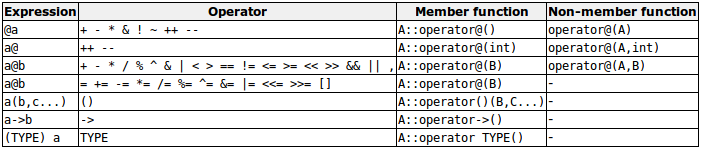
\includegraphics[scale=0.4]{img/OperatorOverload.png}
\end{frame}

\begin{frame}[fragile]{Example}
\begin{lstlisting}
class CVector {
public:
  int x;
  int y;

  CVector() {};

  CVector(int a,int b) : x(a), y(b) {}

  CVector operator+(const CVector& param) {
    CVector temp;
    temp.x = x + param.x;
    temp.y = y + param.y;
    return temp;
  }
};
\end{lstlisting}
\end{frame}

\begin{frame}{Static members}
Static members are `class-members`. They don't belong to an object, but to the
class. Therefore data in static member variables exists only once and static
methods can't access object data.
\end{frame}

\begin{frame}[fragile]{Const member functions}
When an object of a class is qualified as a const object, the access to its data
members from outside the class is restricted to read-only. Methods have to be
devlared as const to make them accessable. Marking all methods that don't modify
the object as const is importent to allow to pass an object as const reference
into a function.

\begin{lstlisting}
class MyClass {
public:
  int x;

  MyClass(int val) : x(val) {}

  int get() const {
    return x;
  }
};

const MyClass foo(10);
int a = foo.x;
int b = foo.get();
\end{lstlisting}

\end{frame}

\subsection{Special members}
\begin{frame}{Special members}
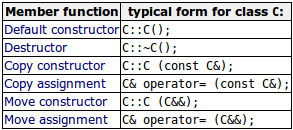
\includegraphics[scale=0.4]{img/SpecialMembers.png}
\end{frame}

\begin{frame}{Default constructors}
The default constructor is the constructor called when objects of a class are
declared, but are not initialized with any arguments. If a class definition has
no constructors, the compiler assumes the class to have an implicitly defined
default constructor.
\end{frame}

\begin{frame}{Destructor}
Destructors fulfill the opposite functionality of constructors: They are
responsible for the necessary cleanup needed by a class when its lifetime ends.
\end{frame}

\begin{frame}{Copy constructor}
A copy constructor is a constructor whose first parameter is of type reference
to the class itself (possibly const qualified) and which can be invoked with a
single argument of this type. 
\par
If a class has no custom copy nor move constructors (or assignments) defined, an
implicit copy constructor is provided. The definition assumed for this function
performs a shallow copy. 
\end{frame}

\begin{frame}[fragile]{Copy assignment}
Objects are not only copied on construction, when they are initialized: They can
also be copied on any assignment operation.
\begin{lstlisting}
MyClass foo;
MyClass bar (foo);  // object init: copy constructor called
MyClass baz = foo;  // object init: copy constructor called
foo = bar;  // object already init: copy assignment called
\end{lstlisting}
\end{frame}

\subsection{Templates}

\begin{frame}{Templates}
Function templates
Class templates
Template specialization
\end{frame}

\section{Other language features}
\subsection{Type conversions}
\begin{frame}[fragile]{Implicit conversion}
Implicit conversions are automatically performed when a value is copied to a
compatible type.
\begin{lstlisting}
short a=2000;
int b;
b=a;
\end{lstlisting}
\end{frame}

\begin{frame}{Implicit conversions with classes}
In the world of classes, implicit conversions can be controlled by means of three member functions:
\begin{itemize}
  \item Single-argument constructors: allow implicit conversion from a
  particular type to initialize an object.
  \item Assignment operator: allow implicit conversion from a particular type on
  assignments.
  \item Type-cast operator: allow implicit conversion to a particular type.
\end{itemize}
\end{frame}

\begin{frame}{Keyword explicit}
On a function call, C++ allows one implicit conversion to happen for each
argument. This may be somewhat problematic for classes, because it is not always
what is intended. But, it can be prevented by marking the affected constructor
with the explicit keyword.

Type-cast member functions can also be specified as explicit. This prevents
implicit conversions in the same way as explicit-specified constructors do for
the destination type.
\end{frame}

\begin{frame}[fragile]{Type casting}
C++ is a strong-typed language. Many conversions, specially those that imply a
different interpretation of the value, require an explicit conversion, known in
C++ as type-casting. There exist two main syntaxes for generic type-casting:
functional and c-like:
\begin{lstlisting}
double x = 10.3;
int y;
y = int (x);  // functional notation
y = (int) x;  // c-like cast notation
\end{lstlisting}
\end{frame}

\begin{frame}{dynamic\_cast}
dynamic\_cast can only be used with pointers and references to classes
(or with void*). Its purpose is to ensure that the result of the type conversion points
to a valid complete object of the destination pointer type.

When dynamic\_cast cannot cast a pointer because it is not a complete object of
the required class it returns a null pointer to indicate the failure.
\end{frame}

\begin{frame}{static\_cast}
static\_cast can perform conversions between pointers to related classes, not
only upcasts (from pointer-to-derived to pointer-to-base), but also downcasts
(from pointer-to-base to pointer-to-derived). No checks are performed during
runtime to guarantee that the object being converted is in fact a full object of
the destination type.
\end{frame}

\begin{frame}{reinterpret\_cast}
reinterpret\_cast converts any pointer type to any other pointer type, even of
unrelated classes. The operation result is a simple binary copy of the value
from one pointer to the other. All pointer conversions are allowed: neither the
content pointed nor the pointer type itself is checked.
\end{frame}

\begin{frame}[fragile]{const\_cast}
This type of casting manipulates the constness of the object pointed by a
pointer, either to be set or to be removed. For example, in order to pass a
const pointer to a function that expects a non-const argument:
\begin{lstlisting}
void print(char * str)
{
  cout << str << '\n';
}

int main() {
  const char* c = "sample text";
  print(const_cast<char *>(c));
  return 0;
}
\end{lstlisting}
\end{frame}

\subsection{Exceptions}
\begin{frame}{Exceptions}
Exceptions provide a way to react to exceptional circumstances (like runtime
errors) in programs by transferring control to special functions called
handlers. 
\end{frame}

\begin{frame}[fragile]{Exceptions}
\begin{lstlisting}
#include <iostream>

int main () {
  try
  {
    throw 20;
  }
  catch (int e)
  {
    std::cout << "An exception occurred. "
                 "Exception Nr. " << e << std::endl;
  }
  return 0;
}
\end{lstlisting}
\end{frame}

\begin{frame}[fragile]{Exceptions}
If an ellipsis (...) is used as the parameter of catch, that handler will catch
any exception no matter what the type of the exception thrown. This can be used
as a default handler that catches all exceptions not caught by other handlers:
\begin{lstlisting}
try {
  // code here
}
catch (int param) { std::cout << "int exception"; }
catch (char param) { std::cout << "char exception"; }
catch (...) { std::cout << "default exception"; }
\end{lstlisting}
\end{frame}

\begin{frame}[fragile]{Standard exceptions}
\begin{lstlisting}
class exception {
public:
  exception () noexcept;
  exception (const exception&) noexcept;
  exception& operator= (const exception&) noexcept;
  virtual ~exception();
  virtual const char* what() const noexcept;
}
\end{lstlisting}
\end{frame}

\begin{frame}{Exceptions thrown by components of the C++ Standard library}
\begin{table}
\begin{tabular}{l | l }
Exception & Description \\
\hline
bad\_alloc & thrown by new on allocation failure \\
bad\_cast & thrown by dynamic\_cast when it fails in a dynamic cast \\
bad\_exception & thrown by certain dynamic exception specifiers \\
bad\_typeid & thrown by typeid \\
bad\_function\_call & thrown by empty function objects \\
bad\_weak\_ptr & thrown by shared\_ptr when passed a bad weak\_ptr
\end{tabular}
\end{table}
\end{frame}

\begin{frame}{Base types for custom exceptions}
Generic exception types that can be inherited by custom exceptions to report
errors.
\begin{table}
\begin{tabular}{l | l }
Exception & Description \\
\hline
logic\_error & error related to the internal logic of the program \\
runtime\_error & error detected during runtime
\end{tabular}
\end{table}
\end{frame}

\subsection{Preprocessor directives}
\begin{frame}{Preprocessor directives}
\begin{itemize}
  \item macro definitions (\#define, \#undef)
  \item Conditional inclusions (\#ifdef, \#ifndef, \#if, \#endif, \#else and \#elif)
  \item Line control (\#line)
  \item Error directive (\#error)
  \item Source file inclusion (\#include)
  \item Pragma directive (\#pragma)
\end{itemize}
\end{frame}

\section{Quirks}

\begin{frame}{Most vexing parse}
% TOOD Most vexing parse
\end{frame}


\part{Generic Programming}

\section{Templates}
\begin{frame}{Templates}
\begin{itemize}
  \item class template
  \item function template
  \item alias template (since C++11)
  \item variable template (since C++14)
\end{itemize}
\end{frame}

\begin{frame}[fragile]{class template}
\begin{lstlisting}
template <typename T, int size>
class Array
{
  T data[size]
};

Array<int, 5> numbers;
Array<char, 10> string;
\end{lstlisting}
\end{frame}

\begin{frame}[fragile]{function template}
\begin{lstlisting}
template <typename T>
T max(T value1, T value2)
{
  if (value1 >= value2)
  {
    return value1;
  }
  else
  {
    return value2;
  }
}

max(5, 8);
max(3.2, 8.7);
\end{lstlisting}
\end{frame}

\subsection{Template specialisation}
\begin{frame}{Full/Partial specialisation}
Any of the following can be fully specialized:
\begin{itemize}
  \item function template
  \item class template 
  \item member function of a class template
  \item static data member of a class template
  \item member class of a class template
  \item member enumeration of a class template
  \item member class template of a class or class template
  \item member function template of a class or class template
\end{itemize}
\end{frame}

\begin{frame}[fragile]{function template}
\begin{lstlisting}
template <typename T>
T max(T value1, T value2);

template <>
bool max(bool value1, bool value2)
{
  return value1 || value2; 
}
\end{lstlisting}
\end{frame}

\begin{frame}[fragile]{class template}
\begin{lstlisting}
template <typename T, int size>
class Array;

template <int size>
class Array<bool, size>
{
  bool data[(size+7)/8];
};
\end{lstlisting}
\end{frame}

\begin{frame}[fragile]{Partial specialisation}
\begin{lstlisting}
template <typename T>
bool max(T value1, T value2);

template <typename T>
T* max(T* value1, T* value2)
{
  if (*value1 <= *value2)
  {
    return value1;
  } 
  else
  {
    return value2;
  }
}

\end{lstlisting}
\end{frame}

\part{C++ and C}
\section{C++ and C}
\begin{frame}{C++ and C}
% TODO C++ and C
\end{frame}


\part{Project organisation}

\section{Organising code in C++}

\begin{frame}{Why bother with organisation?}
\begin{itemize}
  \item speed up compiling time
  \item reduce build dependencies
  \item avoid name clashes
  \item better code management
  \item improves collaborative work
\end{itemize}
\end{frame}

\begin{frame}{One definition rule}
\begin{enumerate}
  \item In any translation unit, a template, type, function or object can have
  no more than one definition.
  \item In the entire program, an object or non-inline function cannot have more
  than one definition.
  \item Some things, like types, templates, and extern inline functions, can be
  defined in more than one translation unit.
\end{enumerate}
\end{frame}

\begin{frame}{Header vs. Source-Files}
\begin{itemize}
  \item [Header] Declarations
  \item [Source] Implementations 
\end{itemize}
A function defined entirely inside a class definition is implicitly an inline
function.
\end{frame}

\begin{frame}{Code organisation}
\begin{itemize}
  \item Each class in it's own file
  \item Each namespace in it's own directory
\end{itemize}
No rule without exception!
\end{frame}


\section{Buildsystem}
\subsection{Tools}
\begin{frame}{Tools}
\begin{description}
  \item[Code:Blocks] \url{http://www.codeblocks.org/}
  \item[Git for Windows] \url{https://git-for-windows.github.io/}
  \item[TortoiseGit] \url{https://tortoisegit.org/}
  \item[CMake] \url{https://cmake.org/}  
\end{description}
\end{frame}


\part{Object Oriented Design}

\section{Basics}

\begin{frame}
Design is all about changable code.
Code is written once, but read many times.
\end{frame}


\section{SOLID}

\begin{frame}{S.O.L.I.D - Principals}
Defined by Robert C. Martin (Oncle Bob)

\begin{description}
\item [S] Single-responsiblity principle
\item [O] Open-closed principle
\item [L] Liskov substitution principle
\item [I] Interface segregation principle
\item [D] Dependency Inversion Principle
\end{description}
\end{frame}

\subsection{Single-responsiblity principle}

\begin{frame}[fragile]{Single-responsiblity principle}
''A class should have only a single responsibility.''
\end{frame}

\begin{frame}[fragile]{SRP - Example}
\begin{lstlisting}[caption=SRP Anti-Example]
class Report
{
  void collectData();
  void print();
};
\end{lstlisting}

\begin{block}{Reasons to change:}
\begin{itemize}
  \item The content of the report could change.
  \item The report format chould change.
\end{itemize}
\end{block}
\end{frame}


\subsection{Open-closed principle}

\begin{frame}{Open-closed principle}
''Software entities (classes, modules, functions, etc.) should be open for
extension, but closed for modification.'
\end{frame}

\begin{frame}[fragile]{OCP - Example}
Adding an new class should lead to no or very little changes at the existing
code.

\begin{lstlisting}[caption=OCP Anti-Example]
class Square {
  float length;
};

class Circle {
  float radius;
};

class AreaCalculator {
  float area(const Square& square) {
    return std::pow(square.length);
  }
  
  float area(const Circle& circle) {
    return std::pow(circle.radius) * M_PI;
  }
};
\end{lstlisting}
\end{frame}

\begin{frame}[fragile]{OCP - Example}
\begin{lstlisting}[caption=OCP Example]
class Shape {
  virtual float area() = 0;
};

class Square : public Shape {
  float length;
  float area() { return std::pow(this->length); }
};

class Circle : public Shape {
  float radius;
  float area() { return std::pow(this->radius) * M_PI; }
};

class AreaCalculator {
  float area(const Shape& shape) { return shape.area(); }
};
\end{lstlisting}
\end{frame}


\subsection{Liskov substitution principle}

\begin{frame}{Liskov substitution principle}
''Subtypes must be substitutable for their base types.''
\end{frame}

\begin{frame}[fragile]{LSP - Example}
\begin{lstlisting}[caption=LSP Example]
class Vehicle {
  virtual void startEngine() {
    // Default engine start functionality
  }
};

class Car : public Vehicle {
  void startEngine() {
    this->engageIgnition();
    Vehicle::startEngine();
  }

  void engageIgnition() {
    // Ignition procedure
  }
};
\end{lstlisting}
Example of LSP Violation: `Square is-a Rectangle`
\end{frame}


\subsection{Interface segregation principle}

\begin{frame}{Interface segregation principle}
''Many client specific interfaces are better than one general purpose
interface''
\end{frame}

\begin{frame}{ISP - Example}
% TODO ISP Example
\end{frame}


\subsection{Dependency Inversion Principle}

\begin{frame}{Dependency Inversion Principle}
Report class depends on DataCollection class by calling data-getters.

If the DataCollection implements a ReportData interface and the Report uses only
this, the two classes are decoupled.
\end{frame}

\section{Programming idiom}
\begin{frame}[fragile]{RAII - Resource Acquisition Is Initialization}
Holding a resource is tied to object lifetime of the `resource handle`.
\par
Resource is allocated during handler construction and released during handler
destruction.

\begin{lstlisting}
class FileHandle {
  std::FILE* file;
public:
  FileHandle(const std::string& filename) {
    file = std::fopen(filename.cstr(), "r");
  }
  
  ~FileHandle() {
    std::fclose(file);
  }
};
\end{lstlisting}
\end{frame}

\section{Pattern}

\begin{frame}{Creational Patterns}
\begin{itemize}
  \item Abstract Factory
  \item Builder
  \item Factory Method
  \item Prototype
  \item Singleton
\end{itemize}
\end{frame}

\begin{frame}{Structural Patterns}
\begin{itemize}
  \item Adapter
  \item Bridge
  \item Composite
  \item Decorator
  \item Façade
  \item Flyweight
  \item Proxy
\end{itemize}
\end{frame}

\begin{frame}{Behavioral Patterns}
\begin{itemize}
  \item Chain of Responsibility
  \item Command
  \item Interpreter
  \item Iterator
  \item Mediator
  \item Memento
  \item Observer
  \item State
  \item Strategy
  \item Template Method
  \item Visitor
\end{itemize}
\end{frame}

\begin{frame}{Build}
Separate the construction of a complex object from its representation so that
the same construction process can create different representations.
\end{frame}

\begin{frame}{Adapter aka Wrapper}
Convert the interface of a class into another interface clients expect. Adapter
lets classes work together that couldn't otherwise because of incompatible
interfaces.
\end{frame}

\part{Clean Code}
\begin{frame}{Express yourself in code}
\url{https://simpleprogrammer.com/2015/04/13/why-comments-are-stupid-a-real-example/}
\end{frame}

\begin{frame}
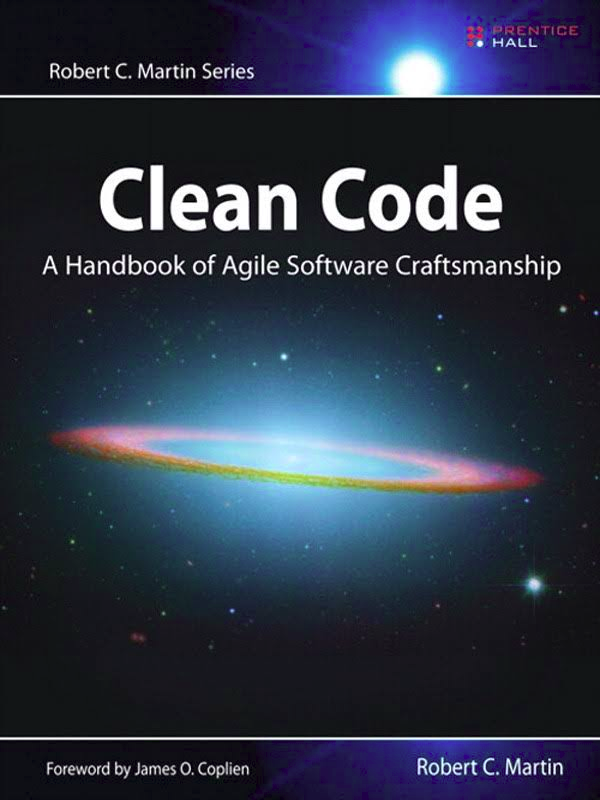
\includegraphics[scale=0.25]{img/CleanCode.png}
\end{frame}

\begin{frame}
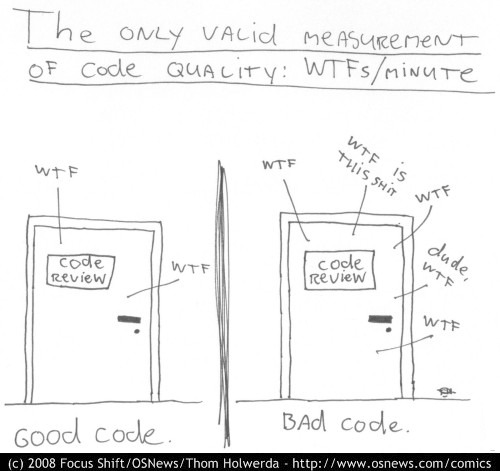
\includegraphics[scale=0.25]{img/wtfm.png}
\end{frame}

\section{Meaningful Names}

\begin{frame}{Meaningful Names}
\begin{exampleblock}{}
  \begin{large}
  ''There are only two hard things in Computer Science: cache
  invalidation and naming things.''
  \end{large}
  \vskip5mm
  \hspace*\fill{\small--- Phil Karlton}
\end{exampleblock}
\end{frame}

\begin{frame}[fragile]{Use Intention-Revealing Names}
\begin{lstlisting}
int d; // elapsed time in days
\end{lstlisting}

\begin{lstlisting}
int elapsedTimeInDays;
\end{lstlisting}
\end{frame}

\begin{frame}{Avoid Disinformation}
\begin{itemize}
  \item Avoid leaving false clues that obscure the meaning of code
  \item Beware of using names which vary in small ways
  \item Use one terminology: Spelling similar concepts similarly
\end{itemize}
\end{frame}

\begin{frame}{Make Meaningful Distinctions}
If names must be different, then they should also mean something different.

Noise words are redundant.
\end{frame}

\begin{frame}[fragile]{Use Pronounceable Names}
Words are, by definition, pronounceable. It would be a shame not to take advantage of that huge portion of our brains that has evolved to deal with spoken lan-
guage. So make your names pronounceable.

\begin{lstlisting}
class DtaRcrd102 {
  Date genymdhms;
  Date modymdhms;
  const String pszqint = "102";
/* ... */
};
\end{lstlisting}

\begin{lstlisting}
class Customer {
  Date generationTimestamp;
  Date modificationTimestamp;
  const String recordId = "102";
/* ... */
};
\end{lstlisting}
\end{frame}

\begin{frame}{Use Searchable Names}
Single-letter names and numeric constants have a particular problem in that they are not
easy to locate across a body of text.
\end{frame}

\begin{frame}{Avoid Encodings}
\begin{itemize}
  \item Hungarian Notation
  \item Member Prefixes
  \item Interfaces and Implementations
\end{itemize}
\end{frame}

\begin{frame}{Avoid Mental Mapping}
Readers shouldn’t have to mentally translate your names into other names they
already know. This problem generally arises from a choice to use neither problem
domain terms nor solution domain terms.
\end{frame}

\begin{frame}[fragile]{Class Names}
Classes and objects should have noun or noun phrase names like
\lstinline{Customer}, \lstinline{WikiPage}, \lstinline{Account}, and
\lstinline{AddressParser}. Avoid words like \lstinline{Manager},
\lstinline{Processor}, \lstinline{Data}, or \lstinline{Info} in the name of a
class. A class name should not be a verb.
\end{frame}

\begin{frame}[fragile]{Method Names}
Methods should have verb or verb phrase names like \lstinline{postPayment},
\lstinline{deletePage}, or \lstinline{save}. Accessors, mutators, and predicates
should be named for their value and prefixed with \lstinline{get},
\lstinline{set} and \lstinline{is}.


When constructors are overloaded, use static factory methods with names that
describe the arguments. For example,
\begin{lstlisting}
Complex* fulcrumPoint = Complex::FromRealNumber(23.0);
\end{lstlisting}
is generally better than
\begin{lstlisting}
Complex* fulcrumPoint = new Complex(23.0);
\end{lstlisting}
\end{frame}

\begin{frame}{Pick One Word per Concept}
Pick one word for one abstract concept and stick with it. For instance, it’s
confusing to have \lstinline{fetch}, \lstinline{retrieve}, and \lstinline{get}
as equivalent methods of different classes.
\end{frame}

\begin{frame}{Separating Solution and Problem Domain}
Separating solution and problem domain concepts is part of the job of a good
programmer and designer. The code that has more to do with problem domain
concepts should have names drawn from the problem domain.
\end{frame}

\begin{frame}{Add Meaningful Context}
Place names in context for your reader by enclosing them in well-named classes,
functions, or namespaces. When all else fails, then prefixing the name may be
necessary as a last resort. 
\end{frame}

\section{Code Smells}
\begin{frame}
    – What? How can code "smell"??

    – Well it doesn't have a nose... but it definitely can stink!

https://sourcemaking.com/refactoring/smells
\end{frame}

\begin{frame}{Bloaters}
\begin{itemize}
  \item Long Method
  \item Large Class
  \item Primitive Obsession
  \item Long Parameter List
  \item Data Clumps
\end{itemize}
\end{frame}

\begin{frame}{Couplers}
\begin{itemize}
  \item Feature Envy
  \item Inappropriate Intimacy
  \item Message Chains
  \item Middle Man
\end{itemize}
\end{frame}

\begin{frame}{Dispensables}
\begin{itemize}
  \item Comments
  \item Duplicate Code
  \item Data Class
  \item Dead Code
  \item Speculative Generality
\end{itemize}
\end{frame}

\begin{frame}{Change Preventers}
\begin{itemize}
  \item Divergent Change
  \item Shotgun Surgery
  \item Parallel Inheritance Hierarchies
\end{itemize}
\end{frame}

\begin{frame}{Object-Orientation Abusers}
\begin{itemize}
  \item Switch Statements
  \item Temporary Field
  \item Refused Bequest
  \item Alternative Classes with Different Interfaces
\end{itemize}
\end{frame}

\begin{frame}[fragile]{Long Method}
A method contains too many lines of code. Generally, any method longer than ten
lines should make you start asking questions.

\begin{lstlisting}
void printOwing() {
  printBanner();

  //print details
  std::cout << "name: " << this->name << std::endl;
  std::cout << "amount: " << getOutstanding() << std::endl;
}
\end{lstlisting}

\begin{lstlisting}
void printOwing() {
  printBanner();
  printDetails(getOutstanding());
}

void printDetails(double outstanding) {
  std::cout << "name: " << this->name << std::endl;
  std::cout << "amount: " << outstanding << std::endl;
}
\end{lstlisting}
\end{frame}

\begin{frame}{Primitive Obsession}
\begin{itemize}
  \item Use of primitives instead of small objects for simple tasks
  \item Use of constants for coding information (such as a constant
  \lstinline{USER_ADMIN_ROLE=1} for referring to users with administrator
  rights.
  \item Use of string constants as field names for use in data arrays.
\end{itemize}
\end{frame}

\begin{frame}[fragile]{Long Parameter List}
More than three or four parameters for a method.
\begin{lstlisting}
struct DateRange
{
public:
    time_t start;
    time_t end;
};

void foo(const DateRange& range)
{
    std::cout << range.start << std::endl;
    std::cout << range.end << std::endl;
}

int main()
{
    DateRange range = {5, 8};
    foo(range);
}
\end{lstlisting}
\end{frame}

\begin{frame}{Data Clumps}
Sometimes different parts of the code contain identical groups of variables
(such as parameters for connecting to a database). These clumps should be turned
into their own classes. 

If you want to make sure whether or not some data is a data clump, just delete
one of the data values and see whether the other values still make sense. If
this is not the case, this is a good sign that this group of variables should be
combined into an object.
\end{frame}

\begin{frame}{Feature Envy}
A method accesses the data of another object more than its own data.
\end{frame}

\begin{frame}{Inappropriate Intimacy}
One class uses the internal fields and methods of another class.
\end{frame}

\begin{frame}{Message Chains}
In code you see a series of calls resembling \lstinline{a->b()->c()->d()}
\end{frame}

\begin{frame}{Middle Man}
If a class performs only one action, delegating work to another class, why does
it exist at all?
\end{frame}

\begin{frame}[fragile]{Comments}
A method is filled with explanatory comments.
\begin{lstlisting}
if (date.before(SUMMER_START) || date.after(SUMMER_END)) {
  // if winter, calculate winter charge
  charge = quantity * winterRate + winterServiceCharge;
}
else {
  // if summer, calculate summer charge
  charge = quantity * summerRate;
}
\end{lstlisting}

\begin{lstlisting}
if (notSummer(date)) {
  charge = winterCharge(quantity);
}
else {
  charge = summerCharge(quantity);
}
\end{lstlisting}
\end{frame}

\begin{frame}{Duplicate Code}
Two code fragments look almost identical.
\end{frame}

\begin{frame}{Data Class}
A data class refers to a class that contains only fields and crude methods for
accessing them (getters and setters). These are simply containers for data used
by other classes. These classes do not contain any additional functionality and
cannot independently operate on the data that they own.  
\end{frame}

\begin{frame}{Dead Code}
A variable, parameter, field, method or class is no longer used (usually because
it is obsolete).

When requirements for the software have changed or corrections have been made,
nobody had time to clean up the old code. 

Such code could also be found in complex conditionals, when one of the branches
becomes unreachable (due to error or other circumstances). 
\end{frame}

\begin{frame}{Speculative Generality}
There is an unused class, method, field or parameter.

Sometimes code is created "just in case" to support anticipated future features
that never get implemented. As a result, code becomes hard to understand and
support.  
\end{frame}

\begin{frame}{Divergent Change}
You find yourself having to change many unrelated methods when you make changes
to a class. For example, when adding a new product type you have to change the
methods for finding, displaying, and ordering products. 
\end{frame}

\begin{frame}{Shotgun Surgery}
Making any modifications requires that you make many small changes to many
different classes.
\end{frame}

\begin{frame}{Parallel Inheritance Hierarchies}
Whenever you create a subclass for a class, you find yourself needing to create
a subclass for another class.
\end{frame}

\begin{frame}[fragile]{Switch Statements}
You have a complex switch operator or sequence of if statements.

\begin{lstlisting}
class Bird {
  //...
  double getSpeed() {
    switch (type) {
      case EUROPEAN:
        return getBaseSpeed();
      case AFRICAN:
        return getBaseSpeed() - getLoadFactor() * numberOfCoconuts;
      case NORWEGIAN_BLUE:
        return (isNailed) ? 0 : getBaseSpeed(voltage);
    }
    throw runtime_exception();
  }
}
\end{lstlisting}
\end{frame}

\begin{frame}[fragile]{Switch Statement}
\begin{lstlisting}
class Bird {
  //...
  virtual double getSpeed() = 0;
}

class European : public Bird {
  double getSpeed() {
    return getBaseSpeed();
  }
}
class African : public Bird {
  double getSpeed() {
    return getBaseSpeed() - getLoadFactor() * numberOfCoconuts;
  }
}
class NorwegianBlue : public Bird {
  double getSpeed() {
    return (isNailed) ? 0 : getBaseSpeed(voltage);
  }
}

// Somewhere in client code
speed = bird.getSpeed();
\end{lstlisting}
\end{frame}

\begin{frame}{Temporary Field}
Temporary fields get their values (and thus are needed by objects) only under
certain circumstances. Outside of these circumstances, they are empty.
\end{frame}

\begin{frame}{Refused Bequest}
If a subclass uses only some of the methods and properties inherited from its
parents, the hierarchy is off-kilter. The unneeded methods may simply go unused
or be redefined and give off exceptions.

Violates `Liskov substitution principle` 
\end{frame}

\begin{frame}{Alternative Classes with Different Interfaces}
Two classes perform identical functions but have different method names.
\end{frame}

\section{Effective C++}

\begin{frame}{Effective C++}
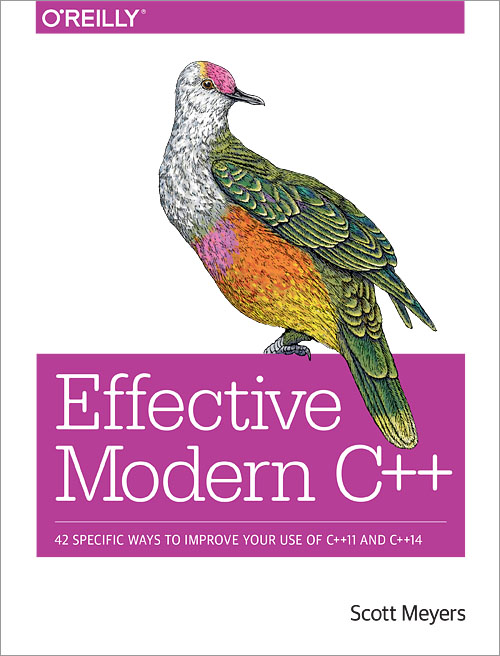
\includegraphics[scale=0.25]{img/EffectiveModernC++.png}
\end{frame}


\part{Coding Standards}

\begin{frame}{Coding Standards}
\begin{itemize}
  \item Roughly 80\% of software defects when using the C or C++ language, are
  attributable to the incorrect usage of 20\% of the language constructs
  \item If the usage of the language can be restricted to avoid this subset that
  is known to be problematic, then the quality of the ensuing software is going
  to greatly increase
\end{itemize}
\begin{center}
\huge If you don’t want defects in your code, then don’t put them there!
\end{center}
\end{frame}

\begin{frame}{Keep It Simple}
\begin{itemize}
  \item It is easy to write code that is difficult to read
  \item Prevent developers from writing `clever` code
  \item Write code that is easy to understand, easy to maintain and easy to test
\end{itemize}
\end{frame}

\begin{frame}[fragile]{Clever Code}
\begin{lstlisting}
void clever_copy(char* to, const char* from, int count)
{
  int n = (count + 7) / 8;
  switch (count % 8 ) {
  case 0: do { *to++ = *from++;
  case 7:      *to++ = *from++;
  case 6:      *to++ = *from++;
  case 5:      *to++ = *from++;
  case 4:      *to++ = *from++;
  case 3:      *to++ = *from++;
  case 2:      *to++ = *from++;
  case 1:      *to++ = *from++;
             } while (--n > 0);
  }
}
\end{lstlisting}

\begin{lstlisting}
void clever_copy(char* to, const char* from, int count)
{
  for (int n = 0; n < count; ++n)
  {
    *to++ = *from++; 
  }
}
\end{lstlisting}
\end{frame}

\begin{frame}{Style guidelines}
\begin{itemize}
  \item Tools can be used to verify coding standards, but there is always a need
  for some manual code review
  \item Style guidelines ensure that the code is always written in the same
  style, facilitating code reviews 
\end{itemize}
\end{frame}


\begin{frame}{Coding Standards can be made up of}
\begin{itemize}
  \item \normalsize Common sense rules \\ \tiny Don’t mix signed and unsigned
  types
  \item \normalsize Reduced language subset \\ \tiny Ensure that 'goto' or
  'malloc' is not used
  \item \normalsize Style guidelines \\ \tiny Ensure that braces are consistent
  placed
  \item \normalsize Naming conventions \\ \tiny Ensure that all public functions
  start with filename\_
  \item \normalsize Quality \& complexity metrics \\ \tiny Ensure that all
  functions have a low cyclomatic complexity
\end{itemize}
\end{frame}


\begin{frame}{Automation}
\begin{itemize}
  \item Use of tools for automation of standards can greatly improve the
  efficiency of their application
  \item Over time engineers will quickly tend to alter their habits and write
  compliant code
  \item Coding Standards should be adopted from the outset of the project
  \item If a coding standard is used with existing code that has a proven track
  record, then the benefits of using the coding standard may be outweighed by
  the risk of introducing defects in making the code compliant!
\end{itemize}
\end{frame}

\begin{frame}{Why Use A Coding Standard?}
\begin{itemize}
  \item Simplest way to avoid numerous potential problems
  \item Mandated by many industrial standards
\end{itemize}
\end{frame}

\begin{frame}{Industry standards}
\begin{block}{DO-178}
Software Consideration in Airborne Systems \& Equipment Certification
\end{block}

\begin{block}{IEC 61508}
Functional Safety of Electrical/Electronic/Programmable Electronic
Safety-related Systems, intended to be a basic functional safety
standard applicable to all kinds of industry
\end{block}

\begin{block}{ISO 26262}
Road vehicles – Functional safety. ISO 26262 is an adaptation of IEC 61508 for
Automotive Electric/Electronic Systems.
\end{block}

\begin{block}{MISRA C / MISRA C++}
Software development guidelines for the C/C++ programming language developed by
MISRA (Motor Industry Software Reliability Association)
\end{block}

\begin{block}{JSF++ AV}
Joint strike fighter air vehicle C++ coding standards for the system
development and demonstration program
\end{block}
\end{frame}


\section{MISRA}
\begin{frame}{MISRA}
\begin{itemize}
  \item It is a language subset
  \item Prevents undefined and unspecified behaviour
  \item Controls implementation-defined behaviour
  \item Gives predictable behaviour
\end{itemize}
\end{frame}

\begin{frame}[fragile]{Undefined behavior}
\begin{lstlisting}
void f(int a, int b, int c)
{ 
  std::cout << "a = " << a 
          << ", b = " << b 
          << ", c = " << c 
          << std::endl; 
}

void main(void)
{
  int i = 0;  
  f(i++, i++, i++); 
}
\end{lstlisting}
\end{frame}

\begin{frame}{Myths and Legends}
\begin{block}{Does NOT}
\begin{itemize}
  \item Say the rules must be followed all the time
  \item Define style or metric guidelines
  \item Stop developers writing code
\end{itemize}
\end{block}
\begin{block}{Does NOT}
\begin{itemize}
  \item Require controlled deviations
  \item Require style and metrics be applied
  \item Force developers to think
\end{itemize}
\end{block}
\end{frame}


\begin{frame}{Examples}
\begin{itemize}
  \item Every defined function shall be called at least once.
  \item There shall be no unused parameters (named or unnamed) in non-virtual
  functions.
  \item Identifiers declared in an inner scope shall not hide an identifier
  declared in an outer scope.
  \item Literal zero (0) shall not be used as the null-pointer-constant.
\end{itemize}
\end{frame}


\part{Testing}

\section{Software Development Process}

\subsection{Models}

\begin{frame}{Waterfall Model}
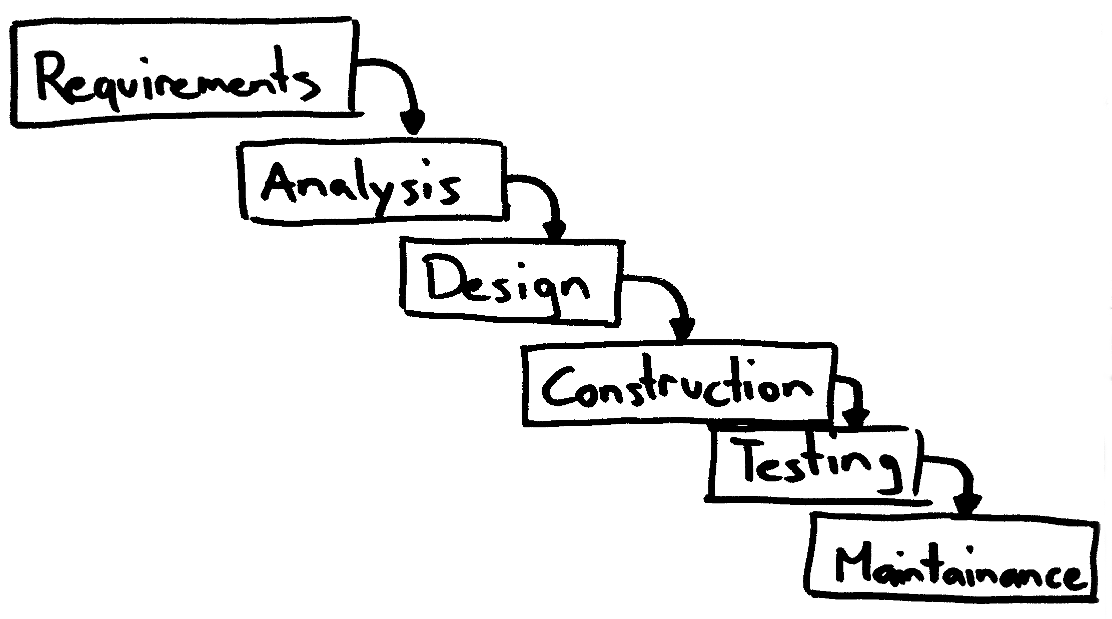
\includegraphics[scale=0.3]{img/Waterfall.png}
\end{frame}

\begin{frame}{Waterfall - Overview}
\begin{enumerate}
  \item System and software requirements: Resulting in product requirements
  \item Analysis: Resulting in models, schema, business rules
  \item Design: Resulting in  the software architecure
  \item Construction: the development, proving, and integration of software
  \item Testing: the systematic discovery and fixing of defects
  \item Maintainance of complete systems
\end{enumerate}
Move to a phase only when its preceding phase is reviewed and verified.
\end{frame}

\begin{frame}{Waterfall}
\begin{itemize}
  \item Places emphasis on documentation
  \item A problem found in the early stages is cheaper to fix
  \item The model provides a structured approach
  \item Requirement changes leads to big redesign
  \item It's hard to do the design for a new problem right
\end{itemize}
\end{frame}

\begin{frame}{V-Model}
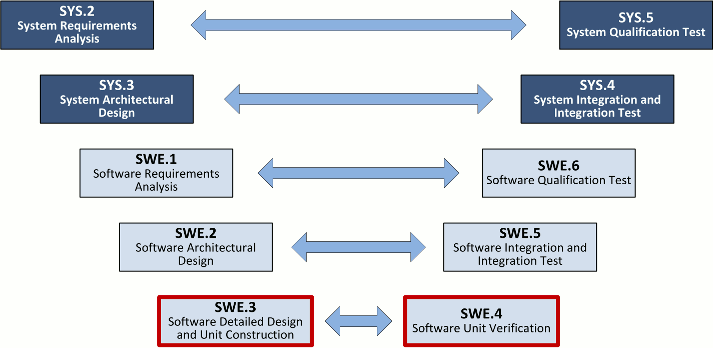
\includegraphics[scale=0.4]{img/VModel.png}
\end{frame}

\begin{frame}{Agile}
\begin{itemize}
  \item \textbf{Individuals and interactions} over processes and tools 
  \item \textbf{Working software} over comprehensive documentation
  \item \textbf{Customer collaboration} over contract negotiation
  \item \textbf{Responding to change} over following a plan
\end{itemize}
\end{frame}

\section{Testing}
\begin{frame}{Testing}
We're talking about automated testing!
\end{frame}

\subsection{Test-pyramid}
\begin{frame}{Test pyramid}
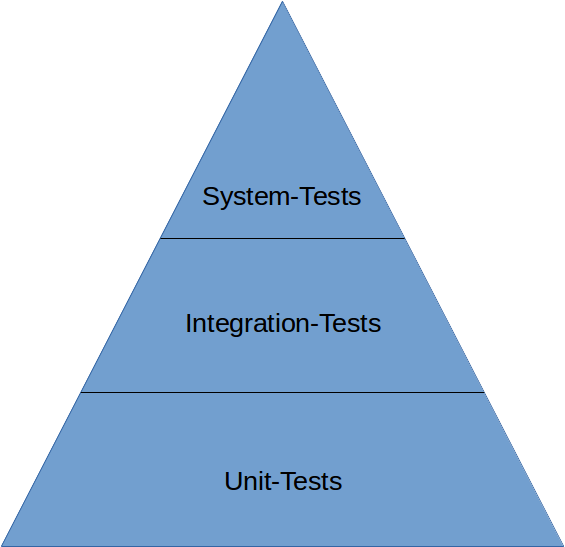
\includegraphics[scale=0.48]{img/TestPyramid.png}
\end{frame}

\begin{frame}{System test}
\begin{itemize}
  \item Test a whole (embedded) system
  \item Often automated in a Hardware-in-the-loop (HIL) system
  \item Blackbox test (internal design is unknown to the tester)
  \item Qualification test (against customer requirements)
\end{itemize}
\end{frame}

\begin{frame}{Integration test}
\begin{itemize}
  \item Test how the single modules (units) are wired
\end{itemize}
\end{frame}

\begin{frame}{Unit test}
\begin{itemize}
  \item Test the behavior of one single translation unit
  \item Test only the public interface
  \item If you think a implementation detail should be tested, then it's perhaps
    it's own unit
\end{itemize}
\end{frame}

\subsection{Design for testability}
\begin{frame}{Design for testability}
\begin{exampleblock}{}
  {\large ``Code that isn't tested doesn't work - this seems to be the safe
  assumption.''}
  \vskip5mm
  
  \hspace*\fill{\small--- Kent Beck}
\end{exampleblock}
\end{frame}

\begin{frame}
Architectural and design decisions in order to enable us to easily and
effectively test our system.
\end{frame}

\subsection{Unit testing}

\begin{frame}{A good test}
\begin{itemize}
  \item Automatic
  \item Thorough
  \item Repeatable
  \item Independent
  \item Professional
  \item Fast
\end{itemize}
\end{frame}

\begin{frame}{3 A's}
\begin{itemize}
  \item Arange
  \item Act
  \item Assert
\end{itemize}
\end{frame}

\begin{frame}[fragile]{Unittesting in C}
Link tests, unit-under-test and test-harness to one executable
\begin{lstlisting}[language=cmake,caption=a unit test in cmake]
add_executable(TestMyModule TestMyModule.cpp MyModule.cpp)
target_link_libraries(TestMyModule gtest gtest_main)
add_test(NAME MyModule COMMAND TestMyModule)
\end{lstlisting}
\end{frame}

\subsection{Test driven development}

\begin{frame}{TDD Cycle}
\begin{enumerate}
  \item Add a test and see it fail (red)
  \item Make your test pass (green)
  \item Refactor code
\end{enumerate}
\end{frame}


\part{Examples}

\section{Exercise 1}
\begin{frame}{Hello World}
\begin{itemize}
  \item Create a `Hello World` application
  \item Create an input for your name and print `Hallo \textit{your name}` 
  \item Simple Calculator: Read two values and print sum
  \item Implement more operations for the calculator
\end{itemize}
\end{frame}

\section{Exercise 2}

\begin{frame}{Smart Pointer}
\subtitle{}
Implement a `Smart Pointer` which handles object-live-time of a newly created
object.
\par
Features:
\begin{itemize}
  \item allocate and free the memory
  \item overload `pointer dereference` operator to access pointee members
  \item implement assignment operator
  \item implement copy operator (with reference counting)
\end{itemize}

\end{frame}

\section{Exercise 3}

\begin{frame}[fragile]{String builder - Background}
Appending to std::string seams a very easy task, but is't very expensiv
regarding performance.

\begin{lstlisting}
std::string text_document;
for (int i=0; i<1000; i++) {
  text_document += line[i];
}
\end{lstlisting}

Every call to append string leads to a new memory allocation and a copy
of the whole string into the new object.
\end{frame}

\begin{frame}[fragile]{String builder - Exercise}
Use the builder pattern to optimize the `expensive` operation of appending text
to an existing string. Use an intermediat buffer to store the string during
creation. Provide functionality to convert the builder object after complete
build into a std::string.

\begin{lstlisting}
StringBuilder str_builder;

for (int i=0; i<1000; i++) {
  str_builder.append("abc");
  // better: str_builder += "abc";
}

std::string str = str_builder.toString();
// better: std::string str = str_builder;
\end{lstlisting}

\end{frame}

\section{Exercise 4}
\begin{frame}[fragile]{Sort adapter}

Create an adapter to use std::sort and std::qsort although they have diverent
interfaces.

\begin{lstlisting}
template <typename T>
class Sorter {
  virtual void operator(T sequence_container) = 0;
}

std::vector seq = {3, 5, 2, 7, 1};

StdlibSorter stdlib_sort;
stdlib_sort(seq);

AlgoSorter algo_sort;
algo_sort(seq);
\end{lstlisting}

\end{frame}

\section{Exercise x}

\begin{frame}{Container}
\begin{itemize}
  \item Singly Linked List
  \item Doubly Linked List
  \item Double Ended Queue
  \item Dynamic Array
  \item Stack (LIFO)
  \item Queue (FIFO)
\end{itemize}
\end{frame}

\end{document}
